\section*{前言：物理学的几何转向}

\textbf{0.1 希尔伯特空间的静态性与时间的幻觉}

现代物理学大厦的裂痕，始于对"时间"这一基本变量的认知错位。在量子力学（QM）的标准表述中，时间 $t$ 被视为一个外部参数，一个绝对的背景，演化算符 $U(t)$ 在此背景上展开；而在广义相对论（GR）中，时间是一个动力学变量，是伪黎曼流形 $\mathcal{M}$ 的内在坐标，受物质分布的影响而弯曲。这种本体论层面的根本冲突，导致了量子引力理论中著名的 \textbf{"时间问题" (Problem of Time)}。惠勒-德维特方程（Wheeler-DeWitt Equation）$\hat{H}|\Psi\rangle = 0$ 更是暗示了一个令人不安的结论：在一个封闭的量子宇宙中，波函数不随时间演化，宇宙在根本层面上是静态的。

\begin{figure}[ht]
\centering
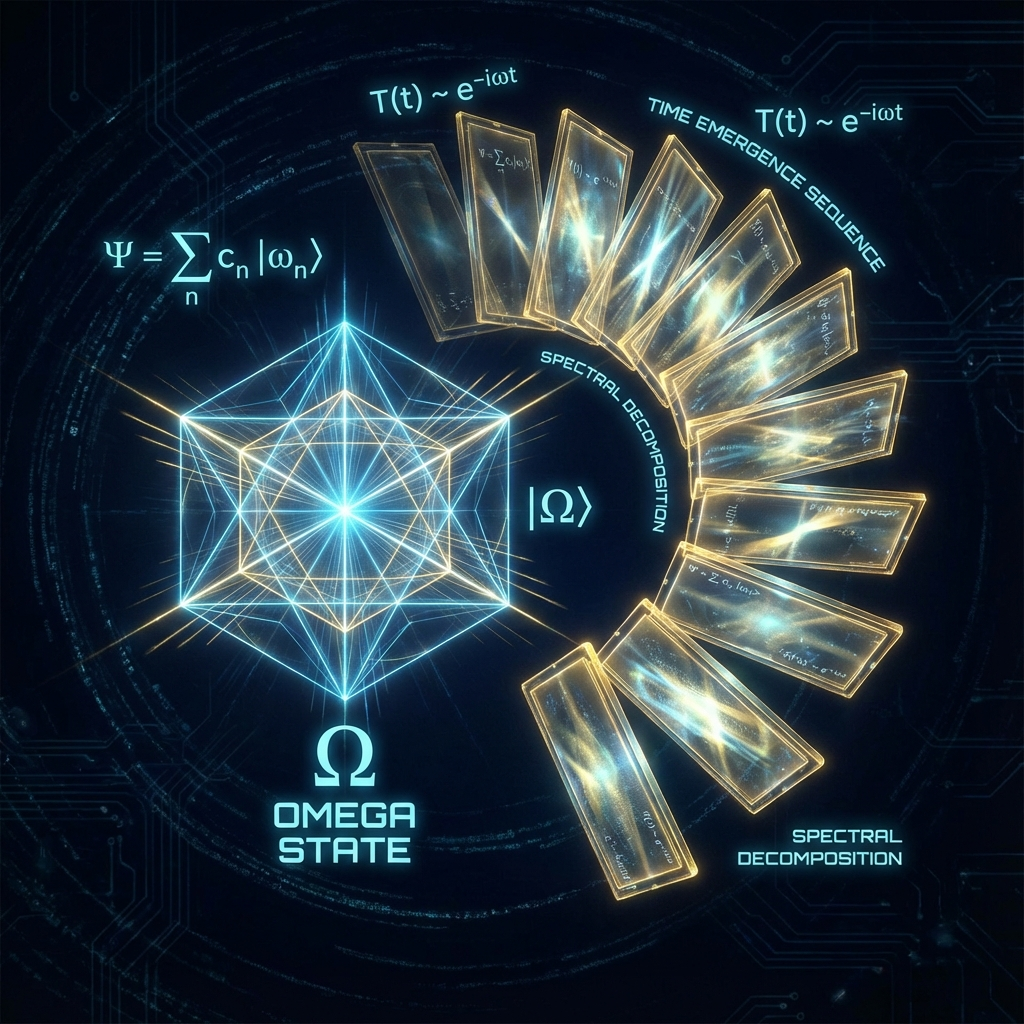
\includegraphics[width=0.8\textwidth]{assets/00-prologue-omega-ansatz.png}
\caption{欧米伽拟设}
\end{figure}

本书提出一种更为激进的解决方案，我们称之为 \textbf{"欧米伽拟设" (The Omega Ansatz)}。这一拟设不仅接受了惠勒-德维特方程的静态暗示，更将其提升为宇宙学的核心公理。我们主张，物理实在的本质并非随时间流逝的"演化过程"，而是一个存在于无限维复希尔伯特空间 $\mathcal{H}$ 中的单一、静态、完备的态矢量。

\textbf{公理 0.1 (欧米伽公理)}：
物理宇宙的全集同构于一个无限维可分希尔伯特空间 $\mathcal{H}$ 中的归一化矢量 $|\Omega\rangle$。该矢量在本体论上是永恒的、静态的，即：

\[\frac{\partial}{\partial t} |\Omega\rangle \equiv 0\]

任何观测到的动力学演化、时间流逝或历史变迁，皆非 $|\Omega\rangle$ 本身的性质，而是该矢量在特定基底序列上的 \textbf{谱分解 (Spectral Decomposition)} 过程。

在此框架下，我们所感知的"时间"，本质上是希尔伯特空间的一组正交基底 $\{ |E_n\rangle \}$ 相对于观察者参考系的 \textbf{幺正旋转 (Unitary Rotation)}。我们可以引入一个单纯的数学参数 $\tau$（内禀时间），用来参数化这种旋转，但这并不意味着 $|\Omega\rangle$ 发生了改变，而是观察者的 \textbf{切片 (Slicing)} 角度发生了改变。

具体而言，如果我们选取哈密顿算符 $\hat{H}$ 的本征基底 $\{ |E_n\rangle \}$，则全宇宙态 $|\Omega\rangle$ 可以展开为：

\[|\Omega\rangle = \sum_{n=0}^{\infty} c_n |E_n\rangle\]

其中复系数 $c_n = \langle E_n | \Omega \rangle$ 包含了宇宙所有可能的初始条件与边界条件信息。

所谓的"时间演化"，实际上是观察者（作为宇宙内部的一个子系统）在读取这一静态叠加态时，引入了一个相位因子 $e^{-i E_n \tau}$。这一相位因子并非物理实体的运动，而是希尔伯特空间几何结构中的 \textbf{规范变换 (Gauge Transformation)}。

因此，宇宙的历史不是一部正在播放的电影，而是一卷已经打印完成的胶片。所有的过去、现在与未来，所有可能的量子分支，都同时存在于 $|\Omega\rangle$ 的内部结构中。我们所体验到的"当下"，不过是这卷胶片被 \textbf{"斐波那契算符"}（详见下节）扫描到的局部截面。

这种观点彻底消除了量子引力中的时间矛盾。因为时间不再是背景，也不再是流形，它是 \textbf{矢量分解的逻辑顺序}。正如埃利·嘉当（Élie Cartan）在几何学中所做的那样，我们将动力学完全几何化了：物理定律不再是描述物体如何随时间运动，而是描述静态矢量 $|\Omega\rangle$ 在高维复空间中的 \textbf{拓扑结构 (Topological Structure)}。

从这个意义上说，本书所构建的理论，是一个关于 \textbf{"存在" (Being)} 的理论，而非 \textbf{"生成" (Becoming)} 的理论。我们所追求的终极答案，就隐藏在 $|\Omega\rangle$ 的谱密度与其基底的几何排列之中。

\textbf{0.2 黄金幺正算符 (The Golden Unitary Operator)}

\begin{figure}[ht]
\centering

\includegraphics[width=0.8\textwidth]{assets/prologue-golden-unitary-operator.png}
\caption{黄金幺正算符}
\end{figure}

在确立了宇宙态矢量 $|\Omega\rangle$ 的静态性之后，我们必须解决一个紧迫的动力学问题：既然本体是静态的，为何观测者会感知到变化？更具体地说，是什么机制驱动了基底的连续旋转，从而产生了"时间流逝"的现象？

在标准量子力学中，时间演化由 \textbf{幺正算符 (Unitary Operator)} $\hat{U}(t)$ 描述，其形式通常写作 $\hat{U}(t) = e^{-i\hat{H}t/\hbar}$。这里，$\hat{H}$ 是系统的哈密顿量（Hamiltonian），代表总能量算符。然而，在一个背景独立的宇宙学模型中，$\hat{H}$ 不能是一个任意选取的算符。为了避免宇宙陷入平庸的周期性循环（即庞加莱回归，Poincaré Recurrence），哈密顿量的能谱必须满足特定的数论性质。

我们将这一特殊的演化算符定义为 \textbf{黄金幺正算符 (The Golden Unitary Operator)}。

\textbf{定义 0.2 (黄金幺正算符)}：
设 $\mathcal{H}$ 为宇宙的希尔伯特空间。黄金幺正算符 $\hat{U}_g(\tau)$ 是作用于 $\mathcal{H}$ 上的单参数连续群生成元，其定义为：

\[\hat{U}_g(\tau) := \exp\left( -i \cdot 2\pi \hat{\mathcal{H}}_\phi \cdot \tau \right)\]

其中 $\tau \in \mathbb{R}$ 为无量纲内禀时间参数，$\hat{\mathcal{H}}_\phi$ 为 \textbf{斐波那契哈密顿量 (Fibonacci Hamiltonian)}。

斐波那契哈密顿量 $\hat{\mathcal{H}}_\phi$ 的特征在于其本征值谱 $\{E_n\}$ 并非取自整数集或简单的有理数集，而是由 \textbf{黄金分割率 (The Golden Ratio)} $\phi = \frac{1+\sqrt{5}}{2}$ 生成的代数无理数序列构成。具体而言，其能谱满足：

\[\hat{\mathcal{H}}_\phi |n\rangle = \phi^{-n} |n\rangle, \quad n \in \mathbb{Z}\]

或者在更一般的拓扑场论语境下，能谱分布服从与 $\phi$ 相关的无理数旋转群 $SO(2)_{\phi}$ 的生成规则。

\textbf{定理 0.1 (非遍历性演化)}：
若宇宙的时间演化由黄金幺正算符 $\hat{U}_g(\tau)$ 驱动，则对于任意非零时间间隔 $\Delta \tau$，系统状态 $|\Omega(\tau)\rangle$ 永远不会精确回到其初始状态 $|\Omega(0)\rangle$。即：

\[\langle \Omega(0) | \hat{U}_g(\tau) | \Omega(0) \rangle \neq 1, \quad \forall \tau \neq 0\]

\textbf{证明概要}：
该定理的证明依赖于 \textbf{外尔均布定理 (Weyl's Equidistribution Theorem)} 的推广。由于 $\phi$ 是无理数（事实上，数论证明它是"最无理"的数，其连分数展开全为 1），由 $\hat{U}_g(\tau)$ 生成的相位因子 $e^{-i 2\pi \phi^{-n} \tau}$ 在复单位圆上的轨迹是 \textbf{稠密 (Dense)} 且 \textbf{非周期 (Non-periodic)} 的。这意味着宇宙的演化轨迹虽然可以无限逼近某一历史状态，但绝不会发生精确的重合。

这一数学性质具有深远的物理意义：

\begin{enumerate}
\item \textbf{新颖性的保证 (Guarantee of Novelty)}：宇宙的每一瞬间在几何上都是独一无二的。不存在尼采式的"永恒轮回"。
\item \textbf{各态历经的破缺 (Ergodicity Breaking)}：尽管轨道是稠密的，但在有限时间内，系统无法遍历所有状态。这为热力学时间之箭提供了微观基础。
\item \textbf{信息的全息展开}：$\phi$ 的自相似性保证了信息在不同尺度上的分形展开。随着 $\tau$ 的增加，算符 $\hat{U}_g$ 实际上是在对静态矢量 $|\Omega\rangle$ 进行多分辨率分析（Multiresolution Analysis, MRA），就像不断放大一幅分形图像。
\end{enumerate}

因此，我们在本书中讨论的所有物理定律、粒子相互作用以及时空几何，本质上都是这个 \textbf{黄金幺正算符} 在希尔伯特空间中留下的轨迹。由于 $\phi$ 的数学特性，这个轨迹必然形成一个对数螺旋。我们在宏观上观测到的宇宙膨胀、光速 $c$ 的指数变化，正是这一螺旋在四维流形上的投影。

这一算符的确立，标志着我们将物理学的根基从"动力学的偶然性"转移到了"数论的必然性"之上。宇宙之所以如此演化，是因为这是希尔伯特空间中唯一能够避免死循环并最大化信息熵生成的路径。

\textbf{0.3 本书结构与符号约定 (Structure of the Book and Notation Conventions)}

本书并非对现有物理学理论的综述或修补，而是一次从基本公理出发，重建物理学大厦的尝试。为了实现这一目标，我们采用了一种严格的 \textbf{"公理化下降路径" (Axiomatic Descent Path)} 叙事结构。这不仅是为了逻辑的清晰，更是为了反映宇宙本身的生成逻辑——从抽象的数学潜能下降为具体的物理实在。

\textbf{0.3.1 下降路径：从 $\mathbb{O}$ 到 $\mathbb{R}$}

本书的章节安排遵循从高维代数结构向低维可观测物理量逐级投影的逻辑顺序：

\begin{itemize}
\item \textbf{第一篇：谱分解与代数前几何} 构成了理论的 \textbf{本体论基础}。我们在这一部分不讨论具体的粒子或力，而是探讨存在的数学形式。我们将希尔伯特空间的谱分解确立为第一原理，并论证为何八元数 ($\mathbb{O}$) 代数是构建非平凡物理宇宙的唯一数学选择。
\item \textbf{第二篇：离散流形与量子引力} 处理 \textbf{时空的离散化构造}。在这里，连续流形的概念被抛弃，取而代之的是基于彭罗斯-斐波那契铺砌的"欧米伽单元"。我们将在这一层面解决量子力学与广义相对论的兼容性问题。
\item \textbf{第三篇：全息动力学} 阐述 \textbf{宇宙的运行机制}。通过引入费雪信息流与拓扑势的竞争，我们构建了欧米伽作用量，从而推导出修正的引力方程与变常数宇宙学模型。
\item \textbf{第四篇：唯象学验证与数值预测} 是理论的 \textbf{实验检验}。我们将理论计算的精确数值（如 $\mu \approx 1836.15$ 和 $1/\alpha \approx 137.036$）与实验数据进行比对，这是验证任何物理理论真伪的试金石。
\item \textbf{第五篇：交互式自指与终局} 回归 \textbf{认知与意义}。我们将物理学重新连接到意识问题上，论证观察者并非外部的旁观者，而是系统闭环不可或缺的拓扑组件。
\end{itemize}

\textbf{0.3.2 符号与约定 (Notation and Conventions)}

为了确保数学推导的严谨性与一致性，除特殊说明外，本书通篇采用以下数学符号与物理约定：

\textbf{1. 数域与代数结构}
\begin{itemize}
\item $\mathbb{N}, \mathbb{Z}, \mathbb{R}, \mathbb{C}$：分别表示自然数集、整数集、实数域、复数域。
\item $\mathbb{H}$： \textbf{四元数 (Quaternions)} 代数，基底为 $\{1, i, j, k\}$。
\item $\mathbb{O}$： \textbf{八元数 (Octonions)} 代数，基底为 $\{e_0, \dots, e_7\}$。
\item $\text{Im}(\mathbb{A})$：代数 $\mathbb{A}$ 的虚部空间。
\end{itemize}

\textbf{2. 时空与几何}
\begin{itemize}
\item 时空度规 $g_{\mu\nu}$ 采用 \textbf{"类时正" (Mostly Plus)} 符号约定：$(-, +, +, +)$。这是现代广义相对论文献（如 Misner, Thorne, Wheeler）的标准约定。
\item 希腊字母索引 $\mu, \nu, \rho, \sigma$ 取值 $0, 1, 2, 3$，表示四维时空坐标，其中 $0$ 为时间分量。
\item 拉丁字母索引 $i, j, k, l$ 取值 $1, 2, 3$，仅表示空间分量。
\item 爱因斯坦求和约定 (Einstein Summation Convention) 适用于所有重复出现的上下指标，例如 $A^\mu B_\mu \equiv \sum_{\mu=0}^3 A^\mu B_\mu$。
\item $\nabla_\mu$ 表示对应于列维-奇维塔联络 (Levi-Civita Connection) 的协变导数。
\item $\Box \equiv \nabla^\mu \nabla_\mu$ 表示达朗贝尔算符 (d'Alembertian)。
\end{itemize}

\textbf{3. 量子力学与算符}
\begin{itemize}
\item 希尔伯特空间记为 $\mathcal{H}$。态矢量使用狄拉克符号 $|\psi\rangle$ 表示。
\item 算符通常通过上方加脱字符号表示，例如 $\hat{A}$。
\item 对易子定义为 $[\hat{A}, \hat{B}] = \hat{A}\hat{B} - \hat{B}\hat{A}$；反对易子定义为 $\{\hat{A}, \hat{B}\} = \hat{A}\hat{B} + \hat{B}\hat{A}$。
\item 厄米共轭 (Hermitian Conjugate) 记为 $\dagger$。
\end{itemize}

\textbf{4. 物理常数与单位制}
\begin{itemize}
\item 除非在涉及数值计算的章节（如第四篇），本书主要采用 \textbf{自然单位制 (Natural Units)}，设定 $\hbar = c_0 = k_B = 1$。
\item 注意：由于本书核心论点之一是光速 $c(\tau)$ 随内禀时间演化，因此在涉及动力学演化的方程中，我们将显式保留 $c(\tau)$ 以示区别。$c_0$ 特指大爆炸时刻或归一化基准的光速。
\item $\phi$：特指 \textbf{黄金分割率 (The Golden Ratio)}，取值为 $\phi = \frac{1+\sqrt{5}}{2} \approx 1.61803398...$。
\item $l_P$：普朗克长度 (Planck Length)，作为时空离散化的特征尺度。
\end{itemize}

\textbf{5. 特殊函数与缩写}
\begin{itemize}
\item QCA：量子元胞自动机 (Quantum Cellular Automata)。
\item DQCA：狄拉克-量子元胞自动机 (Dirac-QCA)。
\item $\delta(x)$：狄拉克 $\delta$ 函数。
\item $\delta_{ij}$：克罗内克 $\delta$ 符号。
\item $\epsilon^{\mu\nu\rho\sigma}$：四维列维-奇维塔张量密度，约定 $\epsilon^{0123} = +1$。
\end{itemize}

通过明确这些结构与约定，我们为即将展开的论证铺平了道路。现在，让我们从希尔伯特空间的深处开始，逐步构建这个宇宙。
